Comparing the performances of our algorithm with the parallel eigenvalue problem solver SLEPc, we compute the same amount of eigenvalues with the same number of processors using the provided Krylov-Schur algorithm \cite{stewart_krylovschur_2002}.
The performances of SLEPc in comparison of our method yields:

\begin{figure}[H]
 \centering
 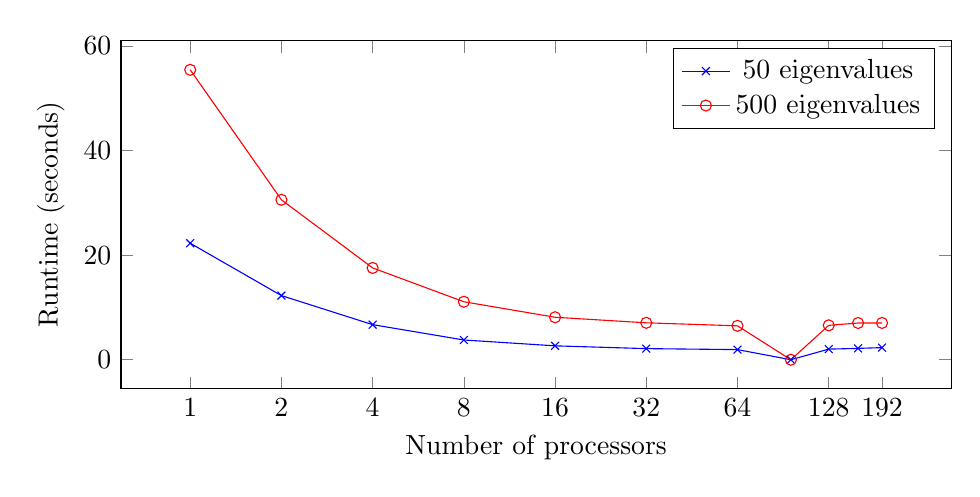
\begin{tikzpicture}
 \begin{axis}[
  height=6cm,
  width=\textwidth,
  xlabel=Number of processors,
  xtick={1, 2, 4, 8, 16, 32, 64, 128, 192},
  xmode=log,
  log ticks with fixed point,
  ylabel=Runtime (seconds)]
   \addplot[color=blue, mark=x] coordinates {
    (1, 22.2659924)
    (2, 12.2595888)
    (4, 6.7051142)
    (8, 3.7737956)
    (16, 2.6544356)
    (32, 2.1228378)
    (64, 1.9344542)
    (96, 0)
    (128, 2.027464)
    (160, 2.1684376)
    (192, 2.3157606)
   };
   \addlegendentry{50 eigenvalues}
   \addplot[color=red, mark=o] coordinates {
    (1, 55.4115932)
    (2, 30.5698838)
    (4, 17.5465694)
    (8, 11.081354)
    (16, 8.1181468)
    (32, 7.0558288)
    (64, 6.4795788)
    (96, 0)
    (128, 6.5703108)
    (160, 7.0204188)
    (192, 7.0297304)
   };
   \addlegendentry{500 eigenvalues}
 \end{axis}
\end{tikzpicture}

 \caption{Runtime of the Krylov-Schur algorithm in SLEPc (log scale).}
 \label{fig:slepc}
\end{figure}

First of all, it is notable that both execution times for 50 and 500 eigenvalues have the same profile and evolve in the same way with respect to the number of processors in figure \ref{fig:slepc}.
The algorithm, for this test case, is faster than our implementation.
However, both approaches tend to have a light increase in the runtime after reaching a certain number of processors.

We should note that SLEPc is a library that has been developed over many years by experts and is specially designed for solving eigenvalue problems in parallel.
It is the current state-of-the-art implementation in this field.
Additionally, the Krylov-Schur algorithm uses a different approach to compute the eigenvalues, so the methods are difficult to compare directly.
